%*******************************************************************************
%****************************** Second Chapter *********************************
%*******************************************************************************

\chapter{Learning Resource Database based on Knowledge Graph}

\ifpdf
    \graphicspath{{Chapter2/Figs/Raster/}{Chapter2/Figs/PDF/}{Chapter2/Figs/}}
\else
    \graphicspath{{Chapter2/Figs/Vector/}{Chapter2/Figs/}}
\fi


\section{Research Motivation}
%在整个推荐系统的各个环节,包括数据收集、数据挖掘和数据推荐,都是以推荐数据源建设为最重要的基石。建立一个精确和完备的题库对于建立一个试题推荐系统是第一步也是重要的一步。题库整体设计的合理性,以及质量,是题库推荐系统成败的关键。题库建设也是一项十分复杂而困难的工作,既是苦活累活又是对教育的理解、技术能力的把握有极高要求的活。在题库建设过程中,并不是简单的数量的堆积,如果不考虑地区差异、应试要求不同和实效性等因素。高中数学学科具有上千规模的知识点,平均每个知识点有从易到难的不同难度的数十道习题,一个优质数学学科题库的规模为十万规模。除去数量上的要求,优质题库除了题目质量,以及对教育内容(教材)的匹配度之外,还有两个根本性问题,其一为知识点关系网络构建,其二为知识点-习题关系构建。而就是对于这些因素的优化,导致了优质题库的建设门槛,以及极高的成本。而市面上的题库往往缺失了对于这些因素的重视,导致出现了许多质量不高的习题数据库。所以,对题目的知识点标签的标注,以及知识体系的构建,是优质题库建设过程中最为核心的问题之一。

%建立试题推荐系统的一个关键问题是如何结合知识点来推荐题目。在考虑这个问题的解决方案的时候,我们首先要考虑的是,我们需要什么样的知识体系和知识点标签。这个问题并不是很容易回答。首先在教材和教学大纲中,以及各种教辅中,会有各种对“知识点”的描述。在高中数学中的知识点,如函数、定义域、值域或解析式等,有直接的概念,也有方法的应用,有专题的抽象,也有相似解法的巧妙汇总,等等——总而言之,这并没有一种标准的体系,就其名称、内涵、粒度、层级,乃至所谓知识点之间的关系或联系,出自各种来源可能是千差万别的。这里既需要教育专家的高屋建瓴,也需要一线教师的灵活经验。其次,作为数据挖掘的任务而言,我们会关心——就标签集合而言,这是一个封闭集还是一个开放集,同时,我们会关心一个“知识点”标签,是一个分类概念还是一个关键词(或者是关键词的组合,短语搭配)。这个定义的明确,对于数据挖掘的问题定义十分关键,也基本决定了后面的方案的选择。但这个明确,不仅要考虑教学意义,同时需要考虑产品对于知识点标签的使用方式,尤其是后者,可能是更加重要的因素。

%作为用于学生的自学推题,并显性化分析报告的试题推荐系统,那么知识点的标签应该要能够描述题目测验的核心知识点、方法或思路,要能够区分对于学生的能力要求点,这样才能构建更为强大的用户模型和推荐引擎,同时报告也方便针对性分析和理解——这个时候需要采取的分类体系和标签集合,其知识点的粒度要足够精细,而知识体系的层级就会大很多,同时,“知识点”即使不是标准体系,也需要大多数的老师和学生认可或一定的使用度。

%在本章中,挖掘的知识点标签,是用于题目的推荐和分析报告。他要求完善题目的知识点关联,即对题目打上若干对应的知识点标签,其中知识点之间也会存在依赖关系,另外就是要建立完整的知识点知识图谱用于生成学生的学习报告。对于第一个问题,它实际上是用题目文本来进行知识点挖掘的任务,也是一个分类任务。具体一点而言,主要是依据题目短文本信息进行层次化分类的任务。在这个任务中,我们需要使用到最基础的技术是自然语言处理和机器学习。也即,通过对大量人工标注好的题目文本和知识点标签结果(也称为训练语料)的学习——通过自然语言处理的技术获取题目文本的特征,通过机器学习来得到分类模型——从而使得系统具有了自动做知识点分类的能力。在这个定义中,待分类对象为题目(包括题干、答案、解析等等),分类结果是一组知识点标签。学习系统的输入就是一组训练语料,即$n$道已经标注好的题目及其对应的知识点标签;学习系统依据这个数据经验,训练出(或学习出)一个模型,这个模型可以是函数表达形式$y=f(x)$,也可以是概率表达形式$p(y|x)$,这个就是学习系统的输出。基于学习系统的分类模型,分类系统就可以做预测,即输入一道新的题目,分类系统自动识别其最可能的知识点标签。第二个问题则是构建一个高中数学知识点知识图谱,它显示了高中数学知识点的结构和关联。通过可视化技术来描述知识资源及其载体,对知识及其相互联系进行挖掘、分析、构建、绘制和显示。同时知识图谱作为人工智能的重要组成部分,目前在推荐系统和问答系统中发挥着越来越重要的作用。另外结合高中数学知识点的关系和学生的学习状态模型,也可以更好地实现学习路径自适应规划。


In all aspects of the whole recommendation system, including data collection, data mining and data recommendation, the construction of the recommendation data source is the most important cornerstone. Establishing an accurate and complete question bank is the first and important step to build a test recommendation system. The reasonableness of the overall design of the question bank, as well as the quality, is the key to the success or failure of the question bank recommendation system. Question bank construction is also a very complex and difficult work, both hard work and the understanding of education, technical ability to grasp a very high demand of work. In the process of building the question bank is not simply the accumulation of quantity, if not take into account regional differences, different test-taking requirements and effectiveness and other factors. High school mathematics subject has thousands of scale of knowledge points, on average, each knowledge point has dozens of exercises from easy to difficult of different difficulty, a quality mathematics subject question bank of 100,000 scale. In addition to the quantitative requirements, there are two fundamental issues for a quality question bank besides the quality of questions and the matching of educational contents (textbooks): one is the construction of knowledge point relationship network, and the other is the construction of knowledge point-exercise relationship. It is the optimization of these factors that leads to the construction threshold of a quality question bank, and the extremely high cost. The question databases on the market often lack the attention to these factors, resulting in many poor-quality exercise databases. Therefore, the labeling of knowledge points of the topics and the construction of knowledge system is one of the most core issues in the process of building a high-quality question database.

One of the key problems in building a test recommendation system is how to recommend topics in conjunction with knowledge points. When considering a solution to this problem, the first thing we need to consider is what kind of knowledge system and knowledge point labels we need. This is not a very easy question to answer. First of all, there are various descriptions of "knowledge points" in textbooks and syllabi, as well as in various teaching aids. In high school mathematics, knowledge points, such as functions, definition domains, value domains, or analytic equations, have direct concepts, applications of methods, abstractions of topics, clever summaries of similar solutions, etc.-in short, there is no standard system of names, connotations, granularity, hierarchy, or even so-called relationships or connections between knowledge points. The names, connotations, granularity, hierarchy, and even the so-called relationships or connections between knowledge points can vary widely from one source to another. Both the high level of educational experts and the flexible experience of frontline teachers are needed here. Second, as a data mining task, we are concerned with - in terms of the set of tags - whether it is a closed set or an open set, and we are concerned with whether a "knowledge point" tag is a categorical concept or a keyword (or a combination of keywords, phrases). combination of keywords, phrase pairing). The clarity of this definition is crucial to the problem definition of data mining and basically determines the choice of the solution that follows. However, this clarity should not only consider the pedagogical significance, but also the way the product uses the knowledge point label, especially the latter, which may be a more important factor.

As a system for students to push questions for self-study and visualize the analysis report, then the tags of knowledge points should be able to describe the core knowledge points, methods or ideas of the topic quiz, and be able to distinguish the ability requirement points for students, so as to build a more powerful user model and recommendation engine, while the report is also convenient for targeted analysis and understanding - this time the classification system and tag collection need to be taken, the granularity of its knowledge points should be fine enough, and the level of the knowledge system will be much larger, at the same time, "knowledge points" even if it is not a standard system, it needs to be recognized by most teachers and students or a certain degree of use.

In this chapter, the knowledge point tags are mined for topic recommendation and analysis reports. He requires to improve the knowledge point association of the topic, i.e., to label the topic with a number of corresponding knowledge points, among which there will also be dependencies between the knowledge points, in addition to establishing a complete knowledge map of knowledge points for generating student learning reports. For the first problem, it is actually a knowledge point mining task using the topic text, which is also a classification task. To be more specific, it is a task of hierarchical classification based on the information in the short text of the topic. In this task, we need to use the most basic technologies of natural language processing and machine learning. That is, by learning a large amount of manually labeled topic text and knowledge point labeling results (also called training corpus) - obtaining the features of the topic text through natural language processing techniques and obtaining the classification model through machine learning - the system The system has the ability to do knowledge point classification automatically. In this definition, the object to be classified is a topic (including stem, answer, paraphrase, etc.), and the result is a set of knowledge point labels. The input of the learning system is a set of training corpus, i.e., $n$ questions that have been labeled and their corresponding knowledge point labels; based on this data experience, the learning system trains (or learns) a model, which can be a functional expression $y=f(x)$ or a probabilistic expression $p(y|x)$, and this is the output of the learning system. Based on the classification model of the learning system, the classification system can then make predictions, i.e., a new topic is entered and the classification system automatically identifies its most likely knowledge labels. The second problem is then to construct a knowledge map of high school mathematics knowledge points, which shows the structure and association of high school mathematics knowledge points. Knowledge resources and their carriers are described through visualization techniques to mine, analyze, construct, map, and display knowledge and its interconnections. Meanwhile knowledge graphs, as an important part of artificial intelligence, are now playing an increasingly important role in recommendation systems and question and answer systems. In addition combining the relationship of high school mathematics knowledge points and students' learning state model, it can also better realize the adaptive planning of learning paths.

\section{Proposed Model}
%在本节中,提出了一个基于图神经网络的模型用于进行试题-知识点关联和知识点知识图谱的建立。该模型大致分为两个部分,第一个部分用一个基于图卷积神经网络半监督学习和文本挖掘嵌入学习的算法来实现的试题-知识点关联模块,用于实现试题知识点标注和关联。第二部分考虑到高中数学的知识的体系化,结合先验领域知识,用改进的R-GCN算法来构建高中数学知识点知识图谱。

In this section, a graph neural network-based model is proposed for test question-knowledge point association and knowledge mapping of knowledge points. The model is roughly divided into two parts. The first part is a test-knowledge point association module implemented with a semi-supervised learning algorithm based on graph convolutional neural networks and text mining embedding learning for test knowledge point labeling and association. The second part considers the systematization of knowledge of high school mathematics and combines a priori domain knowledge with an improved R-GCN algorithm to construct a knowledge graph of high school mathematics knowledge points. 


\subsection{Model Overview}
%本节的任务是构造一个挖掘习题-知识点关系的模型和一个挖掘知识点之间关联的模型。建立习题-知识点关系即对习题进行知识点标注,习题的知识点是理解习题和求解习题所用到的知识概念的集合。所以准确描述一道试题的知识点,对于后续的知识追踪和推荐过程十分重要。一个习题往往具有多个知识点,因此实际上知识点挖掘是一个多标签分类问题\cite{多标签问题},这一点将在后文论述。目前已经存在的基础分类方式有专家标注和机器学习两种方式。前者即教育专家结合自己的专业知识对试题进行知识点标注,但当题量或题目复杂度较高时,人工标注存在工作量大,主观度高和标注不完善等问题。后者则是用机器学习或深度学习的方法,来对习题进行自动知识点标注。因为在习题集中只有少量习题被标注知识点,而其他大量的习题尚未被标注,这些知识点标注往往是半监督或无监督学习的模式。目前往往采用对习题的文本信息挖掘的方式来进行知识点自动标注,考虑到习题推荐

The task of this section is to construct a model for mining the exercise-knowledge point relationship and a model for mining the association between knowledge points. The knowledge point of an exercise is the set of knowledge concepts used to understand the exercise and solve it. So accurately describing the knowledge points of a test question is very important for the subsequent knowledge tracking and recommendation process. An exercise often has multiple knowledge points, so in effect knowledge point mining is a multi-label classification problem \cite {multi-label problem}, as will be discussed later. The two basic classification approaches that already exist are expert labeling and machine learning. The former means that education experts combine their professional knowledge to label the test questions, but when the number of questions or the complexity of the questions is high, manual labeling has problems such as high workload, high subjectivity and imperfect labeling. The latter method uses machine learning or deep learning to automatically annotate the knowledge points of the exercises. Because only a small number of exercises in the exercise set are labeled with knowledge points, while a large number of other exercises are not yet labeled, these knowledge point labeling is often a semi-supervised or unsupervised learning mode. Currently, the text information mining of the exercises is often used to perform automatic knowledge point annotation, considering that the recommendations of the exercises

\subsection{The Knowledge Point Mining of Exercise}


\subsection{The Knowledge Point Relation Mining}


\section{Basic theory of knowledge graph}

%知识图谱是谷歌在2012年提出的一个新概念。知识图本质上是语义网络的知识库,它以结构化的形式描述客观世界中的概念实体及其关系。从一开始的ogle搜索,到现在的聊天机器人、大数据风控、证券投资、智能医疗、自适应教育、推荐系统,都使用了知识图谱。

The Knowledge Graph is a new concept introduced by Google in 2012. Knowledge graph is essentially a knowledge base of Semantic Network, which describes conceptual entities and their relationships in the objective world in a structured form. From the beginning of oogle search, to nowadays chatbots, big data risk control, securities investment, intelligent medical care, adaptive education, recommendation system, all use knowledge graph. 

\subsection{Representation}
Knowledge graphs focus on concepts, entities and their relationships, where entities are things in the objective world and concepts are generalizations and abstractions of things with the same properties. Ontology is the basis of knowledge representation of knowledge graph, which can be formally represented as $O=\{C,H,P,A,I\}$, where $C$ is the set of concepts, such as transactional concepts and event-like concepts, $H$ is the set of contextual relations of concepts, $P$ is the set of attributes, which describes the features possessed by concepts, $A$ is the set of rules, which describes the domain rules, and $I$ is the set of instances, which describes the instance-attribute-value.

The common knowledge graph representations are Resource Description Framework (RDF), Resource Description Framework Schema (RDFS), Web Ontology Language (OWL), etc.

\begin{enumerate}
\item resource description framework RDF is the most commonly used symbolic semantic representation model, which provides a unified standard for describing entities/resources. the basic model of RDF is a directed labeled graph, each edge on the way corresponds to a subject-predicate object triad, and a triad corresponds to a statement of an event. the RDF consists of nodes and edges, the nodes represent entities/resources, attributes, and the edges represent entities and the relationship between entities and attributes. Figure \ref{triad1} shows the relationship between entities and attributes.
\item lightweight schema language RDFS is an extension of RDF by adding the definition of class properties and other Schema layers on top of the objective events provided by RDF. rdfs is mainly used to define term sets, class sets and property sets, mainly including classes, subclasses, properties, subclass properties, domains, scopes and other primitives, which can build the basic class hierarchy and These clauses can build the basic class hierarchy and attribute system.
\item OWL is the core of the Semantic Web technology stack, which provides fast and flexible data modeling capability and efficient automatic reasoning capability.
\end{enumerate}

\begin{figure}[h]
  \centering
  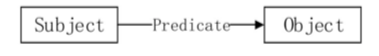
\includegraphics[width=0.8\textwidth]{f01}
  \caption{Structure of Triad}
  \label{triad1}
\end{figure}

\subsection{Storage}
There are mainly two kinds of storage for knowledge graphs, one is based on the academic idea of RDF, which is based on triples car storage: the other is based on the industrial idea of attribute graph, which is based on attribute graph storage.

Using RDF for storage, mainly RDF serialization methods, such as RDF/XML, N- Triples, Turtle, RDFa, JSON-LD, etc.

The most important feature of the graph database for storing knowledge graphs is that the graph database can store not only the nodes and relations of triples, but also the attributes of their nodes and relations together, and the graph can be traversed efficiently, which is convenient for publishing data and retrieval of knowledge graphs.

\section{The construction of knowledge graph}
In order to convert a large number of standard questions into feature questions in a timely manner, this paper proposes an automatic knowledge extraction method based on knowledge graph for test questions. The method uses natural language processing techniques such as named entity recognition, keyword extraction and calculation of semantic similarity of keywords to collect knowledge points and mathematics-related vocabulary in high school mathematics domain and build up a knowledge map of high school mathematics. The mathematics test questions are divided into words and entities by customized dictionaries and rules, and the candidate keywords are extracted and brought into the knowledge map of high school mathematics for querying.

\subsection{The extraction of knowledge point}
In this paper, the architecture for building the knowledge map of high school mathematics is mainly divided into four modules: corpus collection module, pre-processing module, knowledge map building module and knowledge extraction system module. The high school mathematics mapping consists of two entities: mathematical knowledge points and mathematical vocabulary related to mathematical knowledge points, which are mainly used to provide automatic knowledge extraction function for the construction of intelligent question bank later. The question bank not only contains a large number of mathematical knowledge points, but also contains a lot of mathematical vocabulary related to mathematical knowledge points. The mathematical vocabulary does not only stop at the mathematical concept ontology, mathematical textbook chapter names, mathematical knowledge points, etc., but also includes words or vocabulary that can deduce the knowledge points of the test questions. For example, if the operation symbol of "∩" appears in the question, it can be deduced that the question is probably about "set", "set operation", "set intersection operation", "set element interdependence", "set interval", "set interval", "set interval", "set interdependence", "set interval", etc. "The pre-processing module is to standardize the imported data corpus to form structured data, and then to identify the named entities, which mainly involves the process of entity identification and relationship extraction. High school mathematics is relatively a semi-closed and semi-open subject, the mathematical knowledge is relatively closed, but the mathematical test questions are very different, but the final solution still comes back to the test mathematical knowledge, so it is semi-open. The relevant mathematical knowledge points and concepts obtained through knowledge extraction need to be evaluated by experts to create a valuable and credible knowledge map. The knowledge extraction system plays a key role in the construction of the intelligent question bank by tagging the questions obtained by crawlers on the web after processing. 

\subsection{Corpus data preprocessing}
After importing the textbook and web crawler corpus, although a large amount of valuable text, image information and structured data such as question stems and parses in the question bank have been obtained, there are a large number of mathematical formulas in these data, and these mathematical formulas are not standardized because of the platform, and there is no uniform storage format, so it is necessary to standardize these text data containing mathematical formulas.



\begin{itemize}
	\item standardization: The standardization process is mainly for the pictures and mathematical formulas in the corpus, many crawlers get the test information through the pictures, the test information stored in the pictures is very unfavorable to the word separation and naming entity recognition, and the mathematical formulas also exist in a variety of storage methods, currently more common storage and display of mathematical formulas are Office comes with the formula editor plug-in, Mathtype formula editor, Mathml, Latex and so on. For picture information, we use OCR technology for text recognition, and for mathematical formulas, we use Latex format. Mathpix is a software for quickly recognizing mathematical formulas stored in pictures and converting them into Latex format with high recognition accuracy and efficiency, and Latex can extract some useful semantic information for later knowledge extraction when expressing mathematical formulas.
	\item User dictionaries and stopwords: User dictionaries, also known as user-defined dictionaries, are mainly used to enhance the disambiguation and error correction ability of the subscripts by manually adding subscripts rules in the process of named entity recognition, and the subscripts recognition will give priority to the words in the user dictionaries for subscripts after adding the user dictionaries. At present, there is no mature lexical corpus in the field of mathematics, so it is important to build a user lexicon related to mathematics. For example, if we do not add a user lexicon for "function analytic", we will get [function, analytic, equation] if we use the popular third-party corpus Jieba, but we do not want to see such a result when we add the field "analytic" to the user lexicon. When the "parser" field is added to the user's dictionary, the result will be [function,parser]. Deactivated words are also called "dummy words in computer search, non-search words". In search engines, in order to save space and search efficiency, certain words or phrases are usually automatically ignored in search requests, and these words or phrases are called deactivated words. The deactivation dictionary is a filter composed of a number of deactivation words, in the named entity recognition of the word, the system can be based on the deactivation dictionary to filter out some of the words or words that are not useful, to improve the accuracy of the word and the system computing efficiency. Deactivated words mainly include common pronouns, inflectional auxiliaries, adverbs, prepositions, conjunctions, etc., which usually have no obvious meaning of their own and only have a certain role when they are put into a complete sentence, such as: [you, I, he, this, that, the, in, then], etc.
	\item Tokenization: In the process of constructing mathematical knowledge graphs, word separation is mainly used to obtain mathematical knowledge points and related mathematical vocabulary, so there is no strict requirement on the lexicality of the words obtained by word separation. In this paper, we use Hanlp natural language processing toolkit to classify the text by perceptual machine. Hanlp has the features of perfect function, high performance, clear architecture, new corpus and customizable. and can recognize new words
\end{itemize}

\section{Experiment}

\subsection{Dataset and Environment}

The accuracy of the knowledge point extraction directly affects the construction of the feature database. The experiment selected 100,000 and 500 high school mathematics test questions with knowledge points in the web crawler as samples, and divided them into two parts for the automatic extraction of knowledge points without and with expert audit. As shown in Table , the accuracy of knowledge point extraction is 72.3\% when there is no expert review and 96.6\% when there is expert review. This experiment shows that the real-time updating of the knowledge map of high school mathematics in the process of automatic knowledge point extraction is the key to improve the accuracy of knowledge point extraction.

\begin{table}[h]
	\centering

	\begin{tabular}{|l|l|l|}
	\hline
				& Without expert review & With expert review \\ \hline
	Sample Size & 100000                & 500                \\ \hline
	Accuracy    & 72.3\%                & 96.6\%             \\ \hline
	\end{tabular}
	\caption{The accuracy comparison table}
\end{table}

\subsection{Performance Indicators}


\subsection{Design of Experiment}

\subsection{Experiment Review}


\subsection{The Exercise Embedding }

\section{Summary}
This chapter introduces the automatic knowledge extraction method of test questions based on knowledge graph. The intelligent algorithm based on individual features proposes to convert the standard question bank into a feature bank with knowledge feature representation, and defines each dimension in the feature bank, constructs the individual feature bank for users according to individual knowledge points, and explains the recommendation algorithm of test questions in the intelligent question bank; the automatic extraction method of knowledge points of test questions based on knowledge map introduces the whole process of knowledge map of high school mathematics from corpus collection, construction, storage and update. This chapter also introduces the automatic extraction process of knowledge points of high school mathematics test questions. This chapter also presents a comparative experiment on the objectivity of feature database construction and the effectiveness of automatic knowledge point extraction, and the related analysis of the experimental results.